\textbf{{1. 请求分段存储管理系统}}

\textbf{a.
定义:}用户提供了一个比主存可用空间大得多的虚拟存储器。同样,虚拟存储器的实际容量由计算机的地址结构确定。

{\textbf{b.
原理:}请求分段存储管理系统中,作业运行之}{前,\textbf{只要将当前需要的若干段装入主存,便可启动作业运行}。在作业运行过程中,如果要访问的分段不在主存中,则通过调段功能将其调入,同时还可以通过置换功能将暂时不用的分段置换到外存上,以便腾出内存空间。}

{\textbf{c. 段表结构图:}如下图所示。}

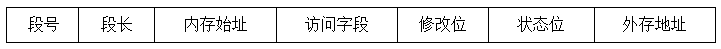
\includegraphics[width=3.33333in,height=0.22917in]{png-jpeg-pics/A9ECDB4463667DDEAB9AA712ED3CF61D.png}

\textbf{变换过程:}段号、段长和内存始址3个信息是进行地址变换所必需的,其他字段的含义与请求分页存储管理相同。当段在内存中时,地址变换过程与分段存储管理相同;当段不在内存中时,应先将该段调入内存,然后再进行地址变换。

\textbf{缺段处理过程:}被访问的段不在主存中时,将产生一个缺段中断信号。操作系统处理该中断时,在主存中查找是否有足够大的分区存放该段。如果没有这样的分区,则检查空闲分区容量总和,确定是否需要对分区进行拼接,或者调出一个或几个段后再装入所需段。
